\documentclass[11pt,openright,a4paper]{report}

%%
%% Package includes to provide the basic style
%%
%%\usepackage{harvard}    % Uses harvard style referencing
\usepackage{graphicx}   % Permits import of various graphics formats
\usepackage{hyperref}   % Provides hyperlinks to sections automatically
\usepackage{pdflscape}  % Provides landscape mode for end code listings
\usepackage{multicol}   % Provides ability to split output into columns
\usepackage{listings}   % Provides styled code listings


%%
%% Set some page size changes from the standard article class
%%
\usepackage{calc}
\setlength{\parskip}{6pt}
\setlength{\parindent}{0pt}
\addtolength{\hoffset}{-0.5cm}
\addtolength{\textwidth}{2.5cm}


%%
%% Format definitions for the style
%%
%%\bibliographystyle{agsm}  %{alpha}
%%\citationstyle{dcu}
\pagestyle{headings}
\fussy


%%
%% Definitions to provide layout in the dissertation title pages
%%
\newenvironment{spaced}[1]
  {\begin{minipage}[c]{\textwidth}\vspace{#1}}
  {\end{minipage}}


\newenvironment{centrespaced}[2]
  {\begin{center}\begin{minipage}[c]{#1}\vspace{#2}}
  {\end{minipage}\end{center}}


\newcommand{\declaration}[2]{
  \thispagestyle{empty}
  \begin{spaced}{4em}
    \begin{center}
      \LARGE\textbf{#1}
    \end{center}
  \end{spaced}
  \begin{spaced}{3em}
    \begin{center}
      Submitted by: #2
    \end{center}
  \end{spaced}
  \begin{spaced}{5em}
    \section*{COPYRIGHT}

    Attention is drawn to the fact that copyright of this dissertation rests
    with its author. The Intellectual Property Rights of the products
    produced as part of the project belong to the author unless otherwise specified
    below, in accordance with the University of Bath's policy on intellectual property 
   (see http://www.bath.ac.uk/ordinances/22.pdf).

    This copy of the dissertation has been supplied on condition that anyone
    who consults it is understood to recognise that its copyright rests with its
    author and that no quotation from the dissertation and no information
    derived from it may be published without the prior written consent of
    the author.

    \section*{Declaration}
    This dissertation is submitted to the University of Bath in accordance
    with the requirements of the degree of Bachelor of Science in the
    Department of Computer Science. No portion of the work in this dissertation
    has been submitted in support of an application for any other degree
    or qualification of this or any other university or institution of learning.
    Except where specifically acknowledged, it is the work of the author.
  \end{spaced}

  \begin{spaced}{5em}
    Signed:
  \end{spaced}
  }


\newcommand{\consultation}[1]{%
\thispagestyle{empty}
\begin{centrespaced}{0.8\textwidth}{0.4\textheight}
\ifnum #1 = 0
This dissertation may be made available for consultation within the
University Library and may be photocopied or lent to other libraries
for the purposes of consultation.
\else
This dissertation may not be consulted, photocopied or lent to other
libraries without the permission of the author for #1 
\ifnum #1 = 1
year
\else
years
\fi
from the date of submission of the dissertation.
\fi
\vspace{4em}

Signed:
\end{centrespaced}
}

%%
%% END OF DEFINITIONS
%%

    %% These are the includes required for the doc 

\usepackage{hyperref}
\usepackage[parfill]{parskip}
\usepackage{csquotes}
\usepackage{graphicx}
\usepackage[toc, page]{appendix}
\usepackage[
  backend=bibtex,
  style=authoryear,
  citestyle=authoryear,
  dateabbrev=false
]{biblatex}

% Fix to apply hyperref to whole biblatex citation instead of just year.
\DeclareCiteCommand{\parencite}[\mkbibparens]
  {\usebibmacro{prenote}}
  {\usebibmacro{citeindex}%
    \printtext[bibhyperref]{\usebibmacro{cite}}}
  {\multicitedelim}
  {\usebibmacro{postnote}}

\DeclareCiteCommand*{\parencite}[\mkbibparens]
  {\usebibmacro{prenote}}
  {\usebibmacro{citeindex}%
    \printtext[bibhyperref]{\usebibmacro{citeyear}}}
  {\multicitedelim}
  {\usebibmacro{postnote}}
% End biblatex fix

\title{Development of an extensible personal informatics system to aid in self management of mental health and wellbeing, making use of both user provided data and user specific API data}
\author{Liam Crewe}
\date{Bachelor of Science in Computer Science with Honours\\University of Bath\\May 2017}

\addbibresource{bibtex.bib} 

\begin{document}

% Set this to the language you want to use in your code listings (if any)
\lstset{language=Java,breaklines,breakatwhitespace,basicstyle=\small}

\setcounter{page}{0}
\pagenumbering{roman}

\maketitle
\newpage


% Set this to the number of years consultation prohibition, or 0 if no limit
\consultation{0}
\newpage


\declaration{Development of an extensible personal informatics system to aid in self management of mental health and wellbeing, making use of both user provided data and user specific API data}{Liam Crewe}
\newpage


\abstract
Your abstract should appear here.  An abstract is a short
paragraph describing the aims of the project, what was
achieved and what contributions it has made.
\newpage


\tableofcontents
\newpage
\listoffigures
\newpage
\listoftables
\newpage


\chapter*{Acknowledgements}
Add any acknowledgements here.
\newpage


\setcounter{page}{1}
\pagenumbering{arabic}

\chapter{Introduction}
\section{Background}
\subsection{Mental Health in the UK}
One in four adults (around 26\%) have been diagnosed with at least one mental health condition \parencite{hse2014} (where adult is any person 16 or over). A further 18\% reported to have experienced a mental health condition but did not seek a diagnosis \parencite{hse2014}. This equates to around 44\% of adults in the UK. The population of the UK is around 65 million \parencite{onspopulation}, of which around 18.8\% are under the age of 16 \parencite{onspopulation}. This equates to a population over the age of 16 of around 81.2\%, or around 52.78 million people. Given that 44\% of these will experience a mental health condition, this equates to over 23 million adults in the UK alone suffering from mental health conditions. This, in addition to any children and young people with mental health conditions truly shows the prevalence of mental health conditions in the UK.

This figure is further supported by the fact that mental health is the result of over 70 million sick days every year \parencite{cmoreport2013}, and is the largest burden of disease with around 28\% of the total burden, compared to 16\% for each of cancer and heart disease \parencite{burdendisorders}. Mental health conditions are estimated to cost the economy between £70 and £100 billion every year \parencite{cmoreport2013}.

\subsection{Mental Health Funding and Capacity}
Despite these figures, the funding for mental health services only sums to around 13\% of total NHS spending \parencite{cepnhsfunding}. In fact, around 75\% of people with mental health conditions receive no treatment at all \parencite{cmoreport2013}. On top of this, although the NHS (National Health Service) is due to receive increased funding in 2016 and the years that follow \parencite{kfnhsbudget}, funding for mental health services is due to rise by just 0.3\% \parencite{mhfunding}. 53 out of 59 services in the UK responded to the freedom of information act made as part of the cited BBC article by \citeauthor{mhfunding}; 23 of which said that their funding would in fact decrease in 2016.

\section{Problem Description}
\subsection{Self Management in Mental Health}
This project is not aiming to find a way to increase the supply of treatment from mental health services, but rather to reduce the demand for it. Much research has been done into the effectiveness of self management for mental health conditions. For example, a study in 2011 tested a particular self management scheme and found that it \enquote{reduces psychiatric symptoms, enhances participants’ hopefulness, and improves their QOL over time} \parencite{wrapstudy}. This shift to self management could help ease the pressure on mental health services, by relieving some of the demand and allowing users to manage their conditions before they worsen. It has also proven particularly effective for relapse prevention in people who have previously undergone treatment for mental health conditions, in that it has been described to \enquote{play a critical role in people's recovery from mental illness} \parencite{selfmanagementrelapse}.

\subsection{Personal Informatics in Mental Health}
This relates to a field known as personal informatics. \enquote{Personal informatics is a class of tools that help people collect personally relevant information for the purpose of self-reflection and self-monitoring} \parencite{personalinformatics}. Personal informatics in mental health is an interesting topic. In 2011 a project aimed to create a personal informatics system that combined sensor data with user inputted data, with the aim of allowing self management of bipolar disorder \parencite{pimentalhealth}. This study found that although personal informatics systems had clear relevance to mental health treatment, little research had been done in the area. It also concluded that the if a system could fuse the collection of personal data into treatment tools in some way, this may have relevance to other mental health disorders, as well as more mild issues such as stress management and the building of balanced, productive lifestyles.

Various applications already exist to allow self management of mental health conditions, such as Optimism \parencite{optimism}. This works by collecting user inputted data and building visualisations the user can look at and draw conclusions from.

While this method of user inputted data works, it is flawed for several reasons. Firstly, users may not be aware of what is a dangerous pattern \parencite{pimentalhealth}, and secondly it requires users to fill in (sometimes lots of) fields fairly frequently. This could lead users to not use the system as often as they could and should. This could be avoided; many modern applications already record data about users, either via user input or automatically. There are many examples of these: mental health apps such as Optimism \parencite{optimism}, fitness apps such as Strava \parencite{strava}, social media apps such as Twitter \parencite{twitter} and many others. This results in a huge amount of data being recorded and made available from applications the user may already use, without requiring the user to submit the data themselves.

This data is very important to this project as mental health is affected by such a wide variety of factors. The examples above for example are discussed below:

\subsubsection{Exercise}
It is common to recommend exercise as a way to help with various mental health conditions. Physical activity is known to alleviate symptoms of mild to moderate depression and has been associated with improvement of self-concept and confidence, as well as reduced symptoms of anxiety \parencite{exercisementalhealth}. Various apps such as Strava \parencite{strava} track how much and how often a user exercises, and could allow the user to correlate exercise frequency and duration with mental health issues.

\subsubsection{Social Media}
It has been shown for example that Facebook can cause depression in some teens when used excessively \parencite{fbdepressionteens}. A research team at Microsoft was even able to build a classifier that used Twitter data to predict onset depressive episodes in patients with major depression, with an accuracy of around 70\% \parencite{de2013predicting}.

\subsection{This Project}
\subsubsection{Overview}
This project aims to take advantage of this data by producing an application called SelfReflect. SelfReflect will only require the user to record a small amount of data about themselves. This will consist of a simple wellbeing questionnaire, which will calculate a wellbeing score. This will then be recorded, along with date and time of submission. The exact nature of this questionnaire will be discussed later, but the key part is that the questionnaire produces a reliable mental health wellbeing score, and is simple, fast and easy for the user to fill out, with the goal that this will allow the user to record their wellbeing more often.

SelfReflect will consist of three distinct parts: a mobile app to allow recording of wellbeing (and automatically date and time of submission), a server side application programming interface (API) to allow storing and retrieval of user data and a web app. The web app will allow the user to add credentials (via the SelfReflect API) to various apps such as Twitter and Strava. This will allow SelfReflect to pull data from these apps via their individual APIs. The web app will then allow the user to interrogate this data and produce visualisations across the multiple data sources.

The goal of this is not to produce a system with an extensive variety of sources and visualisations for the user. Entire projects could be completed on producing lots of different visualisations from just one of these sources with regard to mental health. Instead, SelfReflect will be developed to be extensible; to be built on in the future. Support for two sources (Twitter and Strava) will be developed, with one visualisation for each, as \enquote{proofs of concept}, but this is by no means the final goal of the software system. The API will be built in such a way that a user (or developer) can fetch their data from each source via the SelfReflect API (given that they have provided valid credentials), providing an \enquote{API of APIs}. Also, the API will return \emph{all} data it can access for the user from that source, rather than having one endpoint per visualisation, allowing multiple visualisations to be built from each source in the future.

\section{Aims}
\begin{itemize}
\item Design a system to aid self management of mental health by combining user submitted data with existing applications data., and producing visualisations from this combined data.
\item Design this system to be extensible, so that it can be built on in the future via the addition of more options for sources, more visualisations for new and/or existing sources.
\item Test this system in both a functional and user experience context, including the usability of the various aspects of the system.
\item Investigate the feasibility of this tool as an aid for self management of mental health.
\end{itemize}

\section{Objectives}
\begin{itemize}

\item Design and implement an API that allows:
\begin{itemize}
  \item User creation, log in and management.
  \item Storage of wellbeing score, as well as date and time of submission.
  \item Fetching of user's wellbeing scores over time.
  \item Connection of existing applications (Twitter and Strava) when given valid applications credentials for a user, and storage of these credentials.
  \item Fetching of user's existing application data, to create an \enquote{API of APIs}
\end{itemize} 
  
\item Design and implement a mobile app that allows:
\begin{itemize}
  \item User creation and log in.
  \item Recording of wellbeing score, as well as date and time of submission.
\end{itemize}

\item Design and implement a web application that, via the API disscussed above, allows:
\begin{itemize}
  \item User creation, log in and management.
  \item Recording of wellbeing score, as well as date and time of submission.
  \item Connection of existing applications when given valid applications credentials for a user.
  \item Fetching and combining of user's data from both SelfReflect and connected existing applications, to produce visualisations from this data (one for each of the \enquote{proof of concept} sources.
  \item 
\end{itemize} 

\item Distribute this application to a series of volunteer testers, and get feedback on both the functionality of the system (i.e. if it works) and the usability of the various areas of the system.
\item Analyse the application and the results of the testing to:
\begin{itemize}
  \item Identify possible future changes that could be made and functionality/features that could be added in order to improve the system.
  \item Identify the effectiveness of the sources and visualisations system, and improvements that can be made to it.
  \item Discuss the extensibility of this application for future development.
  \item Discuss the feasibility of this application as a tool for self management of mental health.
\end{itemize}

\end{itemize}

%%%%%%%%%% @TODO:
%% May need to update this later. Depends what goes in each section.
\section{Dissertation Structure}
\textbf{Chapter 1: Introduction}

This chapter provides some high-level background research and motivation for the project, and gives an overview of the project, including its aims and objectives.

\textbf{Chapter 2: Literature Survey}

This chapter delves deeper into the research relevant to this project. It considers relevant literature in terms of motivations and system design, researches methods of recording wellbeing, and compares and contrasts existing applications.

\textbf{Chapter 3: Requirements Specification}

This chapter details the functional and non functional requirements for the system, as derived from the project aims and objectives, and the literature survey. It also discusses the gathering, development and terminology of these requirements.

\textbf{Chapter 4: Design}

This chapter details the design of the three parts of the system (API, mobile app and web app), in order to fulfil the requirements as defined in chapter 3.

\textbf{Chapter 5: Implementation}

This chapter details the implementation of the design as defined in chapter 4.

\textbf{Chapter 6: Testing}

This chapter first discussed automated testing, then continues to detail the methods used for testing functionality, usability and feasibility of the system, using volunteer testers.

\textbf{Chapter 7: Results and Discussion}

This chapter presents the results of the testing by the volunteer testers. It then discusses these results, improvements that could be made to the system based on these results, and the feasibility of the system as a tool to aid in self management of mental health and wellbeing.

\textbf{Chapter 8: Conclusion and Future Work}

This chapter summarises the project and discusses its successes and failures. It also details areas for improvement and for future work.

%%%%%%%%%%

\chapter{Literature Survey}
\section{Introduction} \label{introduction}
This literature survey will identify the various fields this project relates to. It will then present and critique existing work related to these fields, both in the form of academic research and existing technologies. By doing so, it will discuss what exactly this project hopes to contribute to these fields, how it plans to do so, and how this contribution would be useful.

This project encompasses two key fields: personal informatics and mental health. These are two active areas of research, as will be shown and discussed in later sections. This project hopes to combine these two fields in ways that will contribute to them, both in an academic sense, and with the development of a system that could help people to self-manage their mental health effectively. Much existing research will be extremely useful in the design and development of the system, so as to draw on the conclusions of existing work, and make improvements on existing technologies.

\chapter{Requirements Specification}

\ldots


\chapter{Design}

\ldots


\chapter{Implementation}

\ldots


\chapter{Testing}

\ldots


\chapter{Results and Discussion}

\ldots


\chapter{Conclusions and Future Work}

\ldots

\printbibliography

\begin{appendices}
\section{SWEMWBS conversion table} \label{SWEMWBS conversion table}
\begin{figure}[ht]
  \centering
  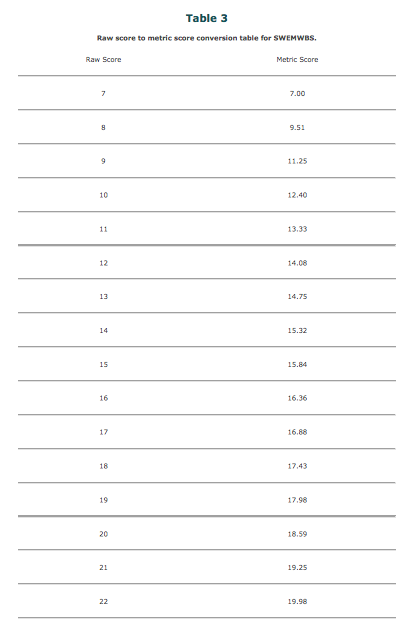
\includegraphics[width =.7\textwidth]{i/swemwbsconversiontable1.png}
  \label{swemwbsconversiontable}
\end{figure}

\begin{figure}[ht]
  \centering
  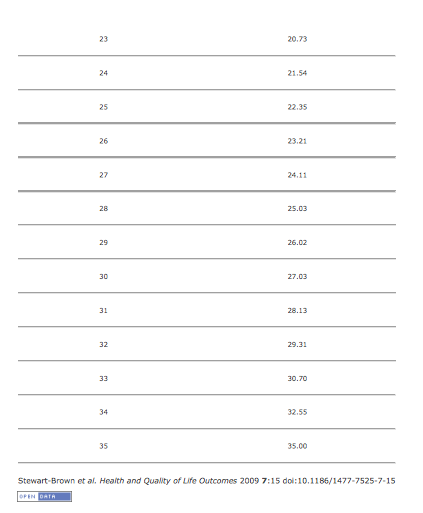
\includegraphics[width =.7\textwidth]{i/swemwbsconversiontable2.png}
\end{figure}
\end{appendices}

\end{document}






%% EXAMPLES

%\chapter{Example Introduction}
%%% Uncomment this to include a separate tex file wih the introduction contents
%%\include{introduction.tex}
%
%This is the introductory chapter.
%
%\section{Example Section}
%Like all chapters, it will have a number of sections
%
%\subsection{Example Subsection}
%\ldots and sub-sections
%
%\subsubsection{Example sub-subsection}
%\ldots and sub-subsections.
%
%\begin{table}[htb]
%\begin{center}
%\caption{An example table}
%\label{Example-Table}
%\begin{tabular}{|l|l|}
%\hline
%Items & Values \\
%\hline
%\hline
%Item 1 & Value 1 \\
%Item 2 & Value 2 \\
%\hline
%\end{tabular}
%\end{center}
%\end{table}
%
%\section[short section title]{Another section}
%Another section, just for good measure.
%You can referene a table, figure or equation using \verb|\ref|, just
%like this reference to table \ref{Example-Table}.
%
%\section{Example lists}
%
%\subsection{Enumerated}
%
%\begin{enumerate}
%\item Example enumerated list
%  \begin{itemize}
%  \item a nested enumerated list item
%  \end{itemize}
%\item Second item in the list
%\end{enumerate}
%
%\subsection{Itemized}
%
%\begin{itemize}
%\item Example itemized list
%  \begin{itemize}
%  \item a nested itemized list item
%  \end{itemize}
%\item Second item in the list
%\end{itemize}
%
%\subsection{Description}
%
%\begin{description}
%\item[Item 1] Example description list
%\item[Item 2] Second item in the list
%\end{description}
%
%
%\chapter{Literature Survey}
%%% Uncomment this to include a separate tex file wih the introduction contents
%%\include{litsurvey.tex}
%This is the chapter for your Literature Survey.
%
%You will wish to cite authors like \parencite{latex} or \parencite{btxdoc}. 
%%Alternate commands are used to cite \citeasnoun{latex} as a noun, or cite
%%\possessivecite{latex} work possessively, or add text to the citation, 
%%\citeaffixed{latex}{e.g.}.
%
%If these citations do not compile correctly, ensure you have the Harvard
%package installed.  You can pick up the Harvard package in the zip file
%of the dissertation template files you downloaded.
%
%
%%%
%%% NOTE: Replace the following with chapters that are appropriate for your
%%%       style of project.  It is unlikely these will fit your project perfectly.
%%%
%
%\chapter{Requirements}
%If you are doing a primarily software development project, this is the
%chapter in which you review the requirements decisions and
%critique the requirements process.
%
%
%\chapter{Design}
%This is the chapter in which you review your design decisions at various
%levels and critique the design process.
%
%
%\chapter{Implementation}
%This is the chapter in which you review the implementation and testing
%decisions and issues, and critique these processes.
%
%Code can be output inline using \verb@\lstinline|some code|@.  For example,
%this code is inline: \lstinline|public static int example = 0;|  (I have
%used the character \verb@|@ as a delimiter, but any non-reserved character
%not in the code text can be used.)
%
%Code snippets can be output using the \verb|\begin{lstlisting} ... \end{lstlisting}|
%environment with the code given in the environment.  For
%example, consider listing \ref{Example-Code}, below.
%
%\begin{lstlisting}[breaklines,breakatwhitespace,caption={Example code},label=Example-Code]
%public static void main() {
%
%  System.out.println("Hello World");
%
%}
%\end{lstlisting}
%
%Code listings are produced using the package ``Listings''.  This has many
%useful options, so have a look at the package documentation for further
%ideas.
%
%\chapter{Testing}
%
%\chapter{Results and Discussion}
%This is the chapter in which you review the outcomes, and
%critique the outcomes process.  You may include user evaluation here
%too.
%
%
%%%
%%% Now we are back to the standard project contents that you should include
%%%
%
%\chapter{Conclusion and Future Work}
%%% Uncomment this to include a separate tex file wih the conclusion contents
%%\include{conclusion.tex}
%
%This is the chapter in which you review the major achievements in the
%light of your original objectives, critique the process, critique your
%own learning and identify possible future work.
%
%\printbibliography
%
%\begin{appendices}
%
%%%
%%% Use the appendix for major chunks of detailed work, such as these. Tailor
%%% these to your own requirements
%%%
%
%\chapter{Design Diagrams}
%
%\chapter{User Documentation}
%
%\chapter{Raw results output}
%
%\chapter{Code}
%
%%%
%%% NOTE that for this to typeset correctly, ensure you use the pdflatex
%%%      command in preference to the latex command.  If you do not have
%%%      the pdflatex command, you will need to remove the landscape and
%%%      multicols tags and just make do with single column listing output
%%%
%
%\begin{landscape}
%\begin{multicols}{2}
%\section{File: yourCodeFile.java}
%\lstinputlisting[basicstyle=\scriptsize]{yourCodeFile.java}
%\end{multicols}
%\end{landscape}
%
%\end{appendices}
%
%\end{document}
